\documentclass[a4paper,twoside,12pt,chapterprefix=false]{scrbook}

\usepackage{amsmath,amssymb,amsthm}
\usepackage{longtable} % tables over several pages
\usepackage[font={small,sl},hang,labelfont=bf]{caption} % configure captions
%\usepackage{captcont} % continue sufigures over several pages
\usepackage{booktabs} % publication quality tables for LaTeX
%\usepackage{showkeys} % shows the labels above the references for easier development

\usepackage{acronym}
\usepackage{subfig}

\ifpdfoutput{%
	\usepackage[pdftex]{graphicx}
	\usepackage[]{pdfpages} %for including full pdf pages
}{%
	\usepackage{graphicx}
}
\usepackage{rotating} % rotate figures

\usepackage{scrpage2}
\KOMAoptions{headinclude}

% Font packages:
\usepackage{times}
\usepackage{helvet}   % sets sans serif font
\usepackage[utf8]{inputenc}

% Listings:
\usepackage{listings}

%PDF hyperref config
\ifpdfoutput{%
	\usepackage[pdftex,
		bookmarks,
		bookmarksopen=true,
		bookmarksnumbered=true,
		pdfauthor={My Name},
		pdftitle={Thesis Title},
		colorlinks,
		linkcolor=black,
		citecolor=black,
		filecolor=black,
		urlcolor=black,
		anchorcolor=black,
		menucolor=black,
		breaklinks=true,
		pageanchor=true,
		plainpages=false,
		pdfpagelabels=true]{hyperref}
}{}

\ifpdfoutput{%
	\pdfcompresslevel=9
	\pdfoutput=1
	\DeclareGraphicsExtensions{.pdf,.png,.eps}
}{}

\bibliographystyle{apalike}

% Uncomment the chapter / section you are working on.
%
%\includeonly{figures}
%\includeonly{tables}
%\includeonly{data-analysis}
%\includeonly{conclusion}
%\includeonly{apx-sample-appendix}

%\pagestyle{useheadings}

% A4
%
\topmargin -0.5in
\textheight 9.3in
\textwidth 6.3in
\oddsidemargin 0.18in
\evensidemargin -0.22in
\parskip 0.1in
\parindent 0in

\renewcommand{\arraystretch}{1.5}
\renewcommand{\baselinestretch}{1}


\begin{document}

%  Terminates current page and paragraph, makes sure next page starts on
%  an odd-number, and generates a completely blank page, without page markers,
%  if necessary.
\newcommand{\clearemptydoublepage}{\newpage{\pagestyle{empty}\cleardoublepage}}



\acrodef{ar}[\textsc{ar}]{Augmented Reality}
\acrodef{vr}[\textsc{vr}]{Virtual Reality}
\acrodef{hmd}[\textsc{hmd}]{Head-Mounted Display}
\acrodef{nes}[\textsc{nes}]{Nintendo Entertainment System}
\acrodef{cmos}[\textsc{cmos}]{Complementary Metal-Oxide-Semiconductor}
\acrodef{ai}[\textsc{ai}]{Artificial Intelligence}
\acrodef{its}[\textsc{its}]{Intelligent Tutoring System}
\acrodef{rpm}[\textsc{rpm}]{revolutions per minute}
\acrodef{zpdes}[\textsc{zpdes}]{Zone of Proximal Development and Empirical Success}
\acrodef{zpd}[\textsc{zpd}]{Zone of Proximal Development}
\acrodef{lod}[\textsc{lod}]{Level of Detail}
\acrodef{dof}[\textsc{dof}]{Degrees of Freedom}
\acrodef{fps}[\textsc{fps}]{Frames per Second}
\acrodef{satnav}[satnav]{Satellite Navigation System}

\newcommand{\refsec}[1]{Section~\ref{sec:#1}}
\newcommand{\refeq}[1]{Eq.~(\ref{eq:#1})}
\newcommand{\reffig}[1]{Figure~\ref{fig:#1}}
\newcommand{\reftab}[1]{Table~\ref{tab:#1}}
\newcommand{\refalg}[1]{Alg.~(\ref{alg:#1})}


\newcommand{\todo}[1]{\textcolor{red}{TODO: #1}}

%% Define leading chapter pages
%
%\addtokomafont{chapter}{\setlength{\parskip}{190pt}}   % SEVERE HACK to keep spacing to chapter art work
\renewcommand*{\chapterheadstartvskip}{\vspace*{215pt}}  % different hack to keep spacing to chapter artwork
%\addtokomafont{chapter}{\rmfamily}        % remove this if you prefer sans-serif section titles
%\addtokomafont{section}{\rmfamily}        % remove this if you prefer sans-serif section titles
%\addtokomafont{subsection}{\rmfamily}     % remove this if you prefer sans-serif section titles
%\addtokomafont{subsubsection}{\rmfamily}  % remove this if you prefer sans-serif section titles
%\addtokomafont{paragraph}{\rmfamily}      % replace by \sffamily if you prefer sans-serif para titles
\addtokomafont{paragraph}{\sffamily}

\def\mychpstyleintl{%
{\noindent\setlength{\tabcolsep}{0pt}\setlength{\arrayrulewidth}{2pt}%
\begin{tabular}{c}
\\[100pt]
\begin{tabular}{lr}
\begin{tabular}{p{0.6\linewidth}}
\\
\end{tabular}
&
\begin{tabular}{p{0.4\linewidth}}
\rightline{{%
\sffamily%
\fontseries{bx}%
\fontshape{n}%
\fontsize{100}{120}%choose baselineskip to be 1.2 times font size
\selectfont
\thechapter}}
\end{tabular}
\end{tabular}\\[300pt]
\end{tabular}
}}

\newpagestyle{mychapterpagestyle}{{\protect\mychpstyleintl}{\protect\mychpstyleintl}}{}
\newpagestyle{myappendixpagestyle}{{\protect\mychpstyleintl}{\protect\mychpstyleintl}}{}
%%


\hypersetup{pageanchor=false} % disabling anchors for title page to avoid warning

%% Replace this by your own design of a title page
%
%\title{Thesis Title}
%\author{My Name}
%\date{September 2042}
%\maketitle
%\clearemptydoublepage
% --- selfmade version ----
\begin{titlepage}
	\topmargin 1.0cm
	\oddsidemargin 0.0cm
	\evensidemargin 0.0cm
	%\textwidth 6.5in
	\centering
	\Huge
	\vspace{3.0cm}
	\textbf{\textsf{Thesis Title}} \\[2.0cm]


	\todo{Put nice teaser image here}


	%\includegraphics*[width=0.4\textwidth]{figures/titlefigure} \\[4.0cm]
	\vspace{5.0cm}
	\sffamily
	\Large
	My Name
	\\[0.8cm]
	\large
	Master Thesis
	\\
	September 2042
	\\[1.3cm]
	Dr. Stéphane Magnenat, Dr. Fabio Zünd\\
	Prof. Dr. Robert W. Sumner
	\vfill
	\includegraphics*[width=0.3\textwidth]{figures/eth_logo_lang_pos} \hfill
	\includegraphics*[width=0.3\textwidth]{figures/GTC_ColorBlack}
	\vspace{3.4cm}
\end{titlepage}
\clearemptydoublepage
%%

\hypersetup{pageanchor=true}
\pagenumbering{roman}
\setcounter{page}{1}

\chapter*{Abstract}
This thesis addresses the development of a novel sample thesis. We analyze the requirements of a general template, as it can be used with the \LaTeX\ text processing system. (And so on\dots) The abstract should not exceed half a page in size!



%include acknowledgment here:
\chapter*{Acknowledgements}
Thank you...

\tableofcontents
\cleardoublepage

\addcontentsline{toc}{chapter}{List of Figures}
\listoffigures
\cleardoublepage

\addcontentsline{toc}{chapter}{List of Tables}
\listoftables
\cleardoublepage

\pagenumbering{arabic}
\renewcommand*{\chapterpagestyle}{mychapterpagestyle}
\renewcommand*{\chapterformat}{} % show chapter titles only (no numbers)
% \setchapterpreamble[o]{...}  unfortunately does not move the \chapter output downwards

% ---- MAIN PART ----

% set counter to n-1:
\setcounter{chapter}{0}

\chapter{Introduction}\label{sec:introduction}


Use acronyms: Novel technology, such as \ac{ar} and \ac{vr}, has ...

\todo{These are todo texts.}

Use references like this: This text is described in more detail in \refsec{introduction} but not in \refsec{relatedwork}. Finally, \reftab{mytable} contains valuable results. For figures with multiple images, you can use \reffig{twofigures} \subref{fig:twofigures:IgeaNarrowBand}.
% set counter to n-1:
\setcounter{chapter}{1}

\chapter{Related Work}\label{sec:relatedwork}


Sample references are~\cite{Zwicker04Perspective} and~\cite{Altman89QuaternionScandal}. 
Lorem ipsum dolor sit amet, consectetuer adipiscing elit, sed diam nonummy nibh euismod tincidunt ut laoreet dolore magna aliquam erat volutpat. Ut wisi enim ad minim veniam, quis nostrud exerci tation ullamcorper suscipit lobortis nisl ut aliquip ex ea commodo consequat. Duis autem vel eum iriure dolor in hendrerit in vulputate velit esse molestie consequat, vel illum dolore eu feugiat nulla facilisis at vero et accumsan et iusto odio dignissim qui.


\section{Appearance Modeling}


Lorem ipsum dolor sit amet, consectetuer adipiscing elit, sed diam nonummy nibh euismod tincidunt ut laoreet dolore magna aliquam erat volutpat. Ut wisi enim ad minim veniam, quis nostrud exerci tation ullamcorper suscipit lobortis nisl ut aliquip ex ea commodo consequat. Duis autem vel eum iriure dolor in hendrerit in vulputate velit esse molestie consequat, vel illum dolore eu feugiat nulla facilisis at vero et accumsan et iusto odio dignissim qui.

\subsection{Taxonomy}

Lorem ipsum dolor sit amet, consectetuer adipiscing elit, sed diam nonummy nibh euismod tincidunt ut laoreet dolore magna aliquam erat volutpat. Ut wisi enim ad minim veniam, quis nostrud exerci tation ullamcorper suscipit lobortis nisl ut aliquip ex ea commodo consequat. Duis autem vel eum iriure dolor in hendrerit in vulputate velit esse molestie consequat, vel illum dolore eu feugiat nulla facilisis at vero et accumsan et iusto odio dignissim qui.

\chapter{Your Central Work}

Always put text between section titles.

\section{Section}

\begin{lstlisting}[mathescape]
$i$ := $0$;
$j$ := $\frac{n}{2}$;
while $i$ $\leq$ $\frac{n}{2}$ and $j$ $\geq$ $0$ do
	if $l_x$[$i$] = b or $l_y$[$j$] = b then
		return true;
	end
	if $l_x$[$i$] + $l_y$[$j$] < b then
		$i$ := $i$ + $1$;
	else if $l_x$[$i$] + $l_y$[$j$] > b then
		$j$ := $j$ - $1$;
	else
		return true;
	end
end
return false;
\end{lstlisting}


\subsection{Another Subsection}

\begin{table}
    \centering
		\caption[Flammkuchenteig]{Flammkuchenteig. The ingredients have to be carefully chosen.\label{tab:mytable}}
    \begin{tabular}{|l|p{0.4\linewidth}|}
    \hline
    \emph{Quant.} & \emph{Ingredient}\\
    \hline
		200g &Wei{\ss}mehl\\
		1/4  &Packung Frischhefe\\
		4EL  &lauwarme Milch\\
		4EL  &Öl\\
		1TL  &Zucker\\
		1TL  &Salz\\
		&lauwarmes Wasser\\
    \hline
    \end{tabular}    
\end{table}

\subsection{More Subsections}


\begin{figure}[htb]
     \centering
     \subfloat[][Caption first]{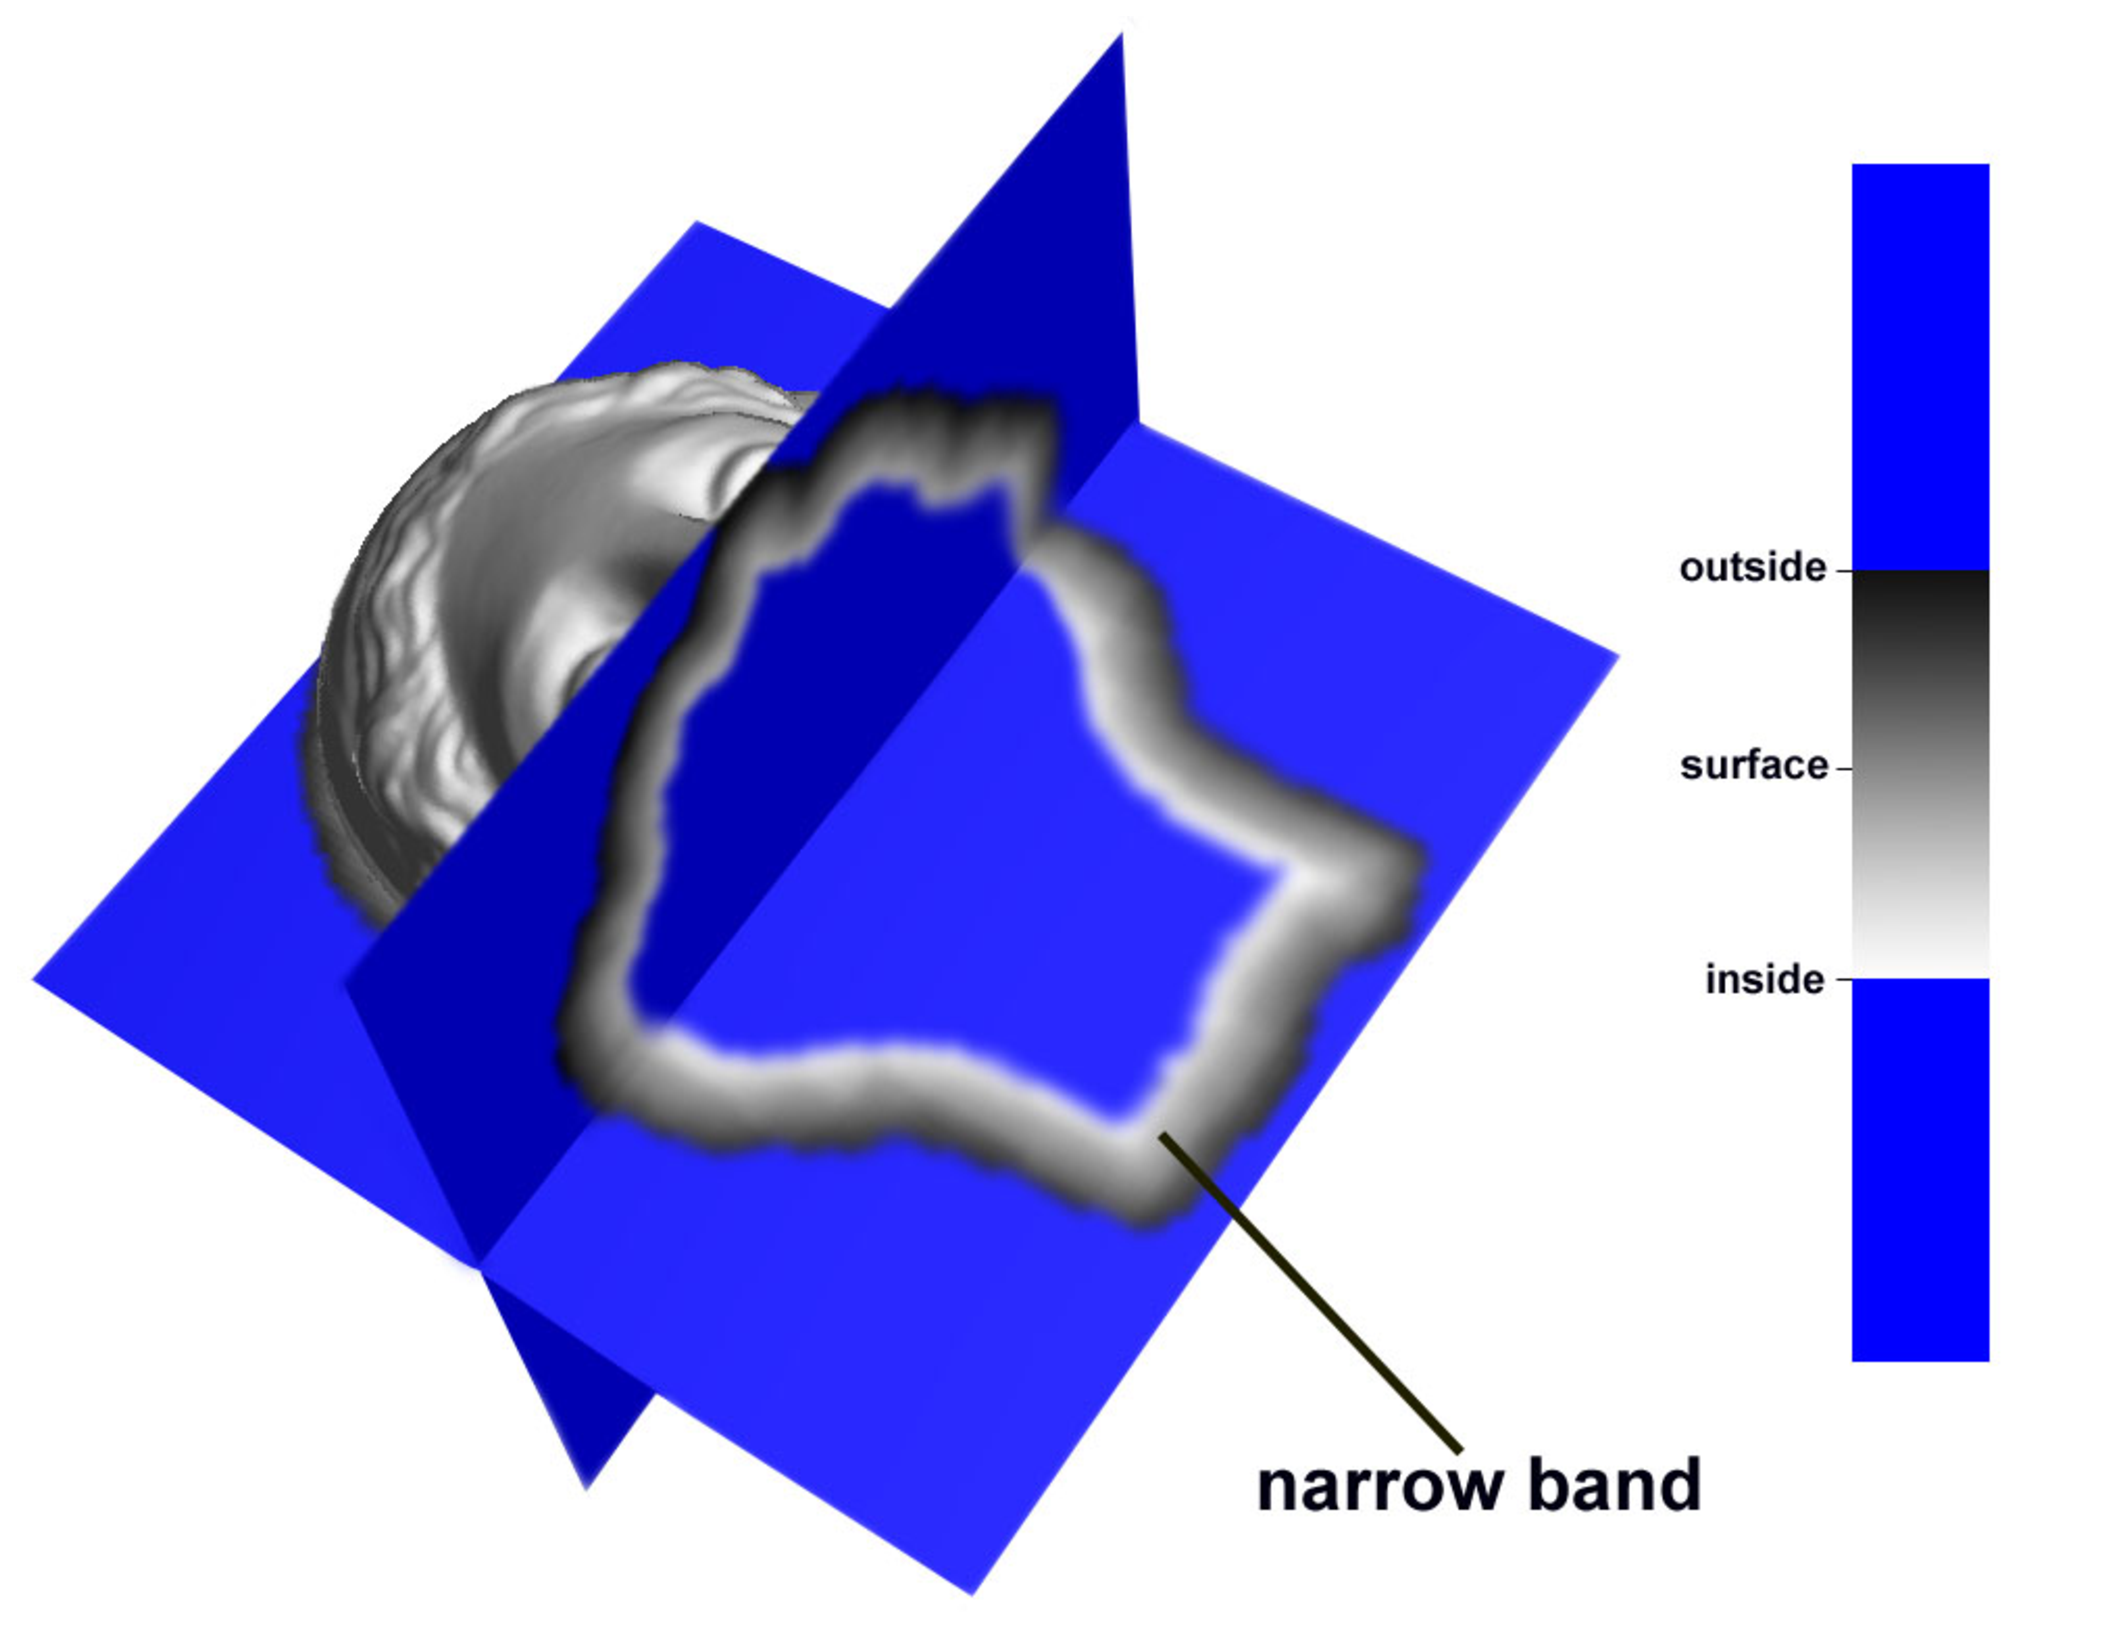
\includegraphics[width=0.45\textwidth]{figures/IgeaNarrowBand}\label{fig:twofigures:IgeaNarrowBand}}
     \subfloat[][Caption first]{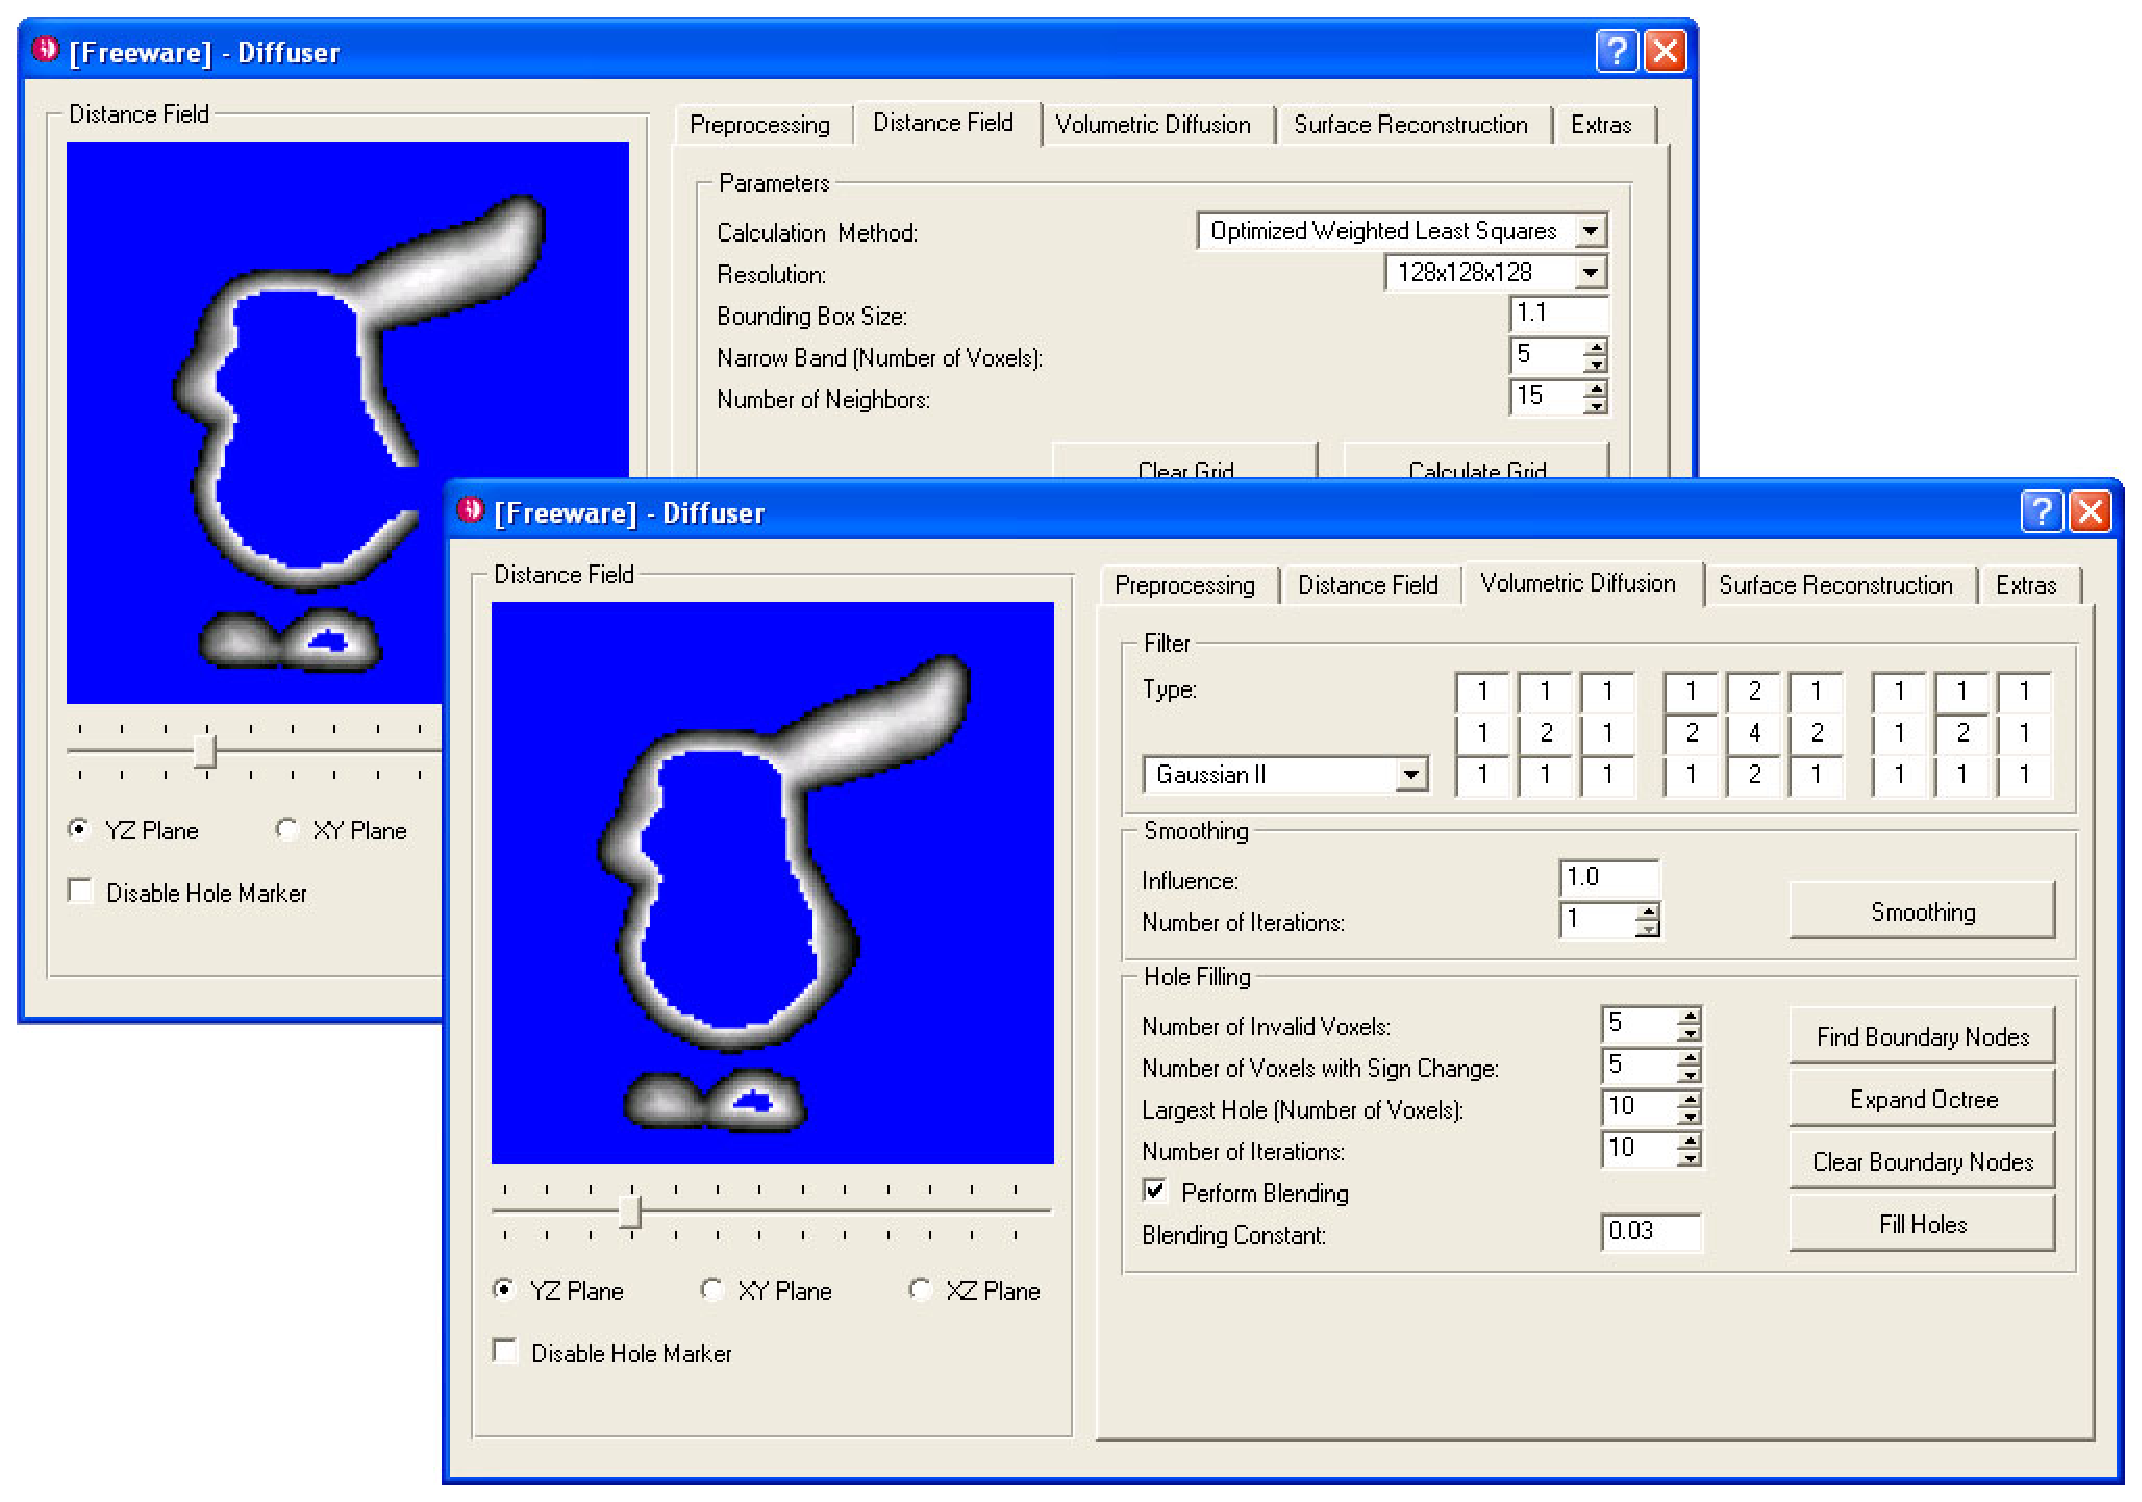
\includegraphics[width=0.45\textwidth]{figures/voldiff_ui}\label{fig:twofigures:voldiff_ui}}
     \caption{Comparison of steady state results. \protect\subref{fig:twofigures:IgeaNarrowBand} x method and \protect\subref{fig:twofigures:voldiff_ui} y method.}
     \label{fig:twofigures}
\end{figure}


\chapter{Results}

Lorem ipsum dolor sit amet, consectetuer adipiscing elit, sed diam nonummy nibh euismod tincidunt ut laoreet dolore magna aliquam erat volutpat. Ut wisi enim ad minim veniam, quis nostrud exerci tation ullamcorper suscipit lobortis nisl ut aliquip ex ea commodo consequat. Duis autem vel eum iriure dolor in hendrerit in vulputate velit esse molestie consequat, vel illum dolore eu feugiat nulla facilisis at vero et accumsan et iusto odio dignissim qui blandit praesent luptatum zzril delenit augue duis dolore te feugait nulla facilisi. Lorem ipsum dolor sit amet, consectetuer adipiscing elit, sed diam nonummy nibh euismod tincidunt ut laoreet dolore magna aliquam erat volutpat. Ut wisi enim ad minim veniam, quis nostrud exerci tation ullamcorper suscipit lobortis nisl ut aliquip ex ea commodo consequat. Duis autem vel eum iriure dolor in hendrerit in vulputate velit esse molestie consequat, vel illum dolore eu feugiat nulla facilisis at vero et accumsan et iusto odio dignissim qui blandit

Lorem ipsum dolor sit amet, consectetuer adipiscing elit, sed diam nonummy nibh euismod tincidunt ut laoreet dolore magna aliquam erat volutpat. Ut wisi enim ad minim veniam, quis nostrud exerci tation ullamcorper suscipit lobortis nisl ut aliquip ex ea commodo consequat. Duis autem vel eum iriure dolor in hendrerit in vulputate velit esse molestie consequat, vel illum dolore eu feugiat nulla facilisis at vero et accumsan et iusto odio dignissim qui blandit praesent luptatum zzril delenit augue duis dolore te feugait nulla facilisi. Lorem ipsum dolor sit amet, consectetuer adipiscing elit, sed diam nonummy nibh euismod tincidunt ut laoreet dolore magna aliquam erat volutpat. Ut wisi enim ad minim veniam, quis nostrud exerci tation ullamcorper suscipit lobortis nisl ut aliquip ex ea commodo consequat. Duis autem vel eum iriure dolor in hendrerit in vulputate velit esse molestie consequat, vel illum dolore eu feugiat nulla facilisis at vero et accumsan et iusto odio dignissim qui blandit
Lorem ipsum dolor sit amet, consectetuer adipiscing elit, sed diam nonummy nibh euismod tincidunt ut laoreet dolore magna aliquam erat volutpat. Ut wisi enim ad minim veniam, quis nostrud exerci tation ullamcorper suscipit lobortis nisl ut aliquip ex ea commodo consequat. Duis autem vel eum iriure dolor in hendrerit in vulputate velit esse molestie consequat, vel illum dolore eu feugiat nulla facilisis at vero et accumsan et iusto odio dignissim qui blandit praesent luptatum zzril delenit augue duis dolore te feugait nulla facilisi. Lorem ipsum dolor sit amet, consectetuer adipiscing elit, sed diam nonummy nibh euismod tincidunt ut laoreet dolore magna aliquam erat volutpat. Ut wisi enim ad minim veniam, quis nostrud exerci tation ullamcorper suscipit lobortis nisl ut aliquip ex ea commodo consequat. Duis autem vel eum iriure dolor in hendrerit in vulputate velit esse molestie consequat, vel illum dolore eu feugiat nulla facilisis at vero et accumsan et iusto odio dignissim qui blandit

Lorem ipsum dolor sit amet, consectetuer adipiscing elit, sed diam nonummy nibh euismod tincidunt ut laoreet dolore magna aliquam erat volutpat. Ut wisi enim ad minim veniam, quis nostrud exerci tation ullamcorper suscipit lobortis nisl ut aliquip ex ea commodo consequat. Duis autem vel eum iriure dolor in hendrerit in vulputate velit esse molestie consequat, vel illum dolore eu feugiat nulla facilisis at vero et accumsan et iusto odio dignissim qui blandit praesent luptatum zzril delenit augue duis dolore te feugait nulla facilisi. Lorem ipsum dolor sit amet, consectetuer adipiscing elit, sed diam nonummy nibh euismod tincidunt ut laoreet dolore magna aliquam erat volutpat. Ut wisi enim ad minim veniam, quis nostrud exerci tation ullamcorper suscipit lobortis nisl ut aliquip ex ea commodo consequat. Duis autem vel eum iriure dolor in hendrerit in vulputate velit esse molestie consequat, vel illum dolore eu feugiat nulla facilisis at vero et accumsan et iusto odio dignissim qui blandit

\chapter{Conclusion}

Lorem ipsum dolor sit amet, consectetuer adipiscing elit, sed diam nonummy nibh euismod tincidunt ut laoreet dolore magna aliquam erat volutpat. Ut wisi enim ad minim veniam, quis nostrud exerci tation ullamcorper suscipit lobortis nisl ut aliquip ex ea commodo consequat. Duis autem vel eum iriure dolor in hendrerit in vulputate velit esse molestie consequat, vel illum dolore eu feugiat nulla facilisis at vero et accumsan et iusto odio dignissim qui blandit praesent luptatum zzril delenit augue duis dolore te feugait nulla facilisi. Lorem ipsum dolor sit amet, consectetuer adipiscing elit, sed diam nonummy nibh euismod tincidunt ut laoreet dolore magna aliquam erat volutpat. Ut wisi enim ad minim veniam, quis nostrud exerci tation ullamcorper suscipit lobortis nisl ut aliquip ex ea commodo consequat. Duis autem vel eum iriure dolor in hendrerit in vulputate velit esse molestie consequat, vel illum dolore eu feugiat nulla facilisis at vero et accumsan et iusto odio dignissim qui blandit

Lorem ipsum dolor sit amet, consectetuer adipiscing elit, sed diam nonummy nibh euismod tincidunt ut laoreet dolore magna aliquam erat volutpat. Ut wisi enim ad minim veniam, quis nostrud exerci tation ullamcorper suscipit lobortis nisl ut aliquip ex ea commodo consequat. Duis autem vel eum iriure dolor in hendrerit in vulputate velit esse molestie consequat, vel illum dolore eu feugiat nulla facilisis at vero et accumsan et iusto odio dignissim qui blandit praesent luptatum zzril delenit augue duis dolore te feugait nulla facilisi. Lorem ipsum dolor sit amet, consectetuer adipiscing elit, sed diam nonummy nibh euismod tincidunt ut laoreet dolore magna aliquam erat volutpat. Ut wisi enim ad minim veniam, quis nostrud exerci tation ullamcorper suscipit lobortis nisl ut aliquip ex ea commodo consequat. Duis autem vel eum iriure dolor in hendrerit in vulputate velit esse molestie consequat, vel illum dolore eu feugiat nulla facilisis at vero et accumsan et iusto odio dignissim qui blandit
Lorem ipsum dolor sit amet, consectetuer adipiscing elit, sed diam nonummy nibh euismod tincidunt ut laoreet dolore magna aliquam erat volutpat. Ut wisi enim ad minim veniam, quis nostrud exerci tation ullamcorper suscipit lobortis nisl ut aliquip ex ea commodo consequat. Duis autem vel eum iriure dolor in hendrerit in vulputate velit esse molestie consequat, vel illum dolore eu feugiat nulla facilisis at vero et accumsan et iusto odio dignissim qui blandit praesent luptatum zzril delenit augue duis dolore te feugait nulla facilisi. Lorem ipsum dolor sit amet, consectetuer adipiscing elit, sed diam nonummy nibh euismod tincidunt ut laoreet dolore magna aliquam erat volutpat. Ut wisi enim ad minim veniam, quis nostrud exerci tation ullamcorper suscipit lobortis nisl ut aliquip ex ea commodo consequat. Duis autem vel eum iriure dolor in hendrerit in vulputate velit esse molestie consequat, vel illum dolore eu feugiat nulla facilisis at vero et accumsan et iusto odio dignissim qui blandit


\section{Future Work}

Lorem ipsum dolor sit amet, consectetuer adipiscing elit, sed diam nonummy nibh euismod tincidunt ut laoreet dolore magna aliquam erat volutpat. Ut wisi enim ad minim veniam, quis nostrud exerci tation ullamcorper suscipit lobortis nisl ut aliquip ex ea commodo consequat. Duis autem vel eum iriure dolor in hendrerit in vulputate velit esse molestie consequat, vel illum dolore eu feugiat nulla facilisis at vero et accumsan et iusto odio dignissim qui blandit praesent luptatum zzril delenit augue duis dolore te feugait nulla facilisi. Lorem ipsum dolor sit amet, consectetuer adipiscing elit, sed diam nonummy nibh euismod tincidunt ut laoreet dolore magna aliquam erat volutpat. Ut wisi enim ad minim veniam, quis nostrud exerci tation ullamcorper suscipit lobortis nisl ut aliquip ex ea commodo consequat. Duis autem vel eum iriure dolor in hendrerit in vulputate velit esse molestie consequat, vel illum dolore eu feugiat nulla facilisis at vero et accumsan et iusto odio dignissim qui blandit



% ---- END MAIN PART ----


\appendix
\clearpage
\renewcommand*{\chapterpagestyle}{myappendixpagestyle}

\chapter{Information For The Few}



\section{A Long Table with Booktabs}


{\scriptsize
\begin{longtable}{clccccccc}
\caption[wordlist]{A sample list of words.}\\
\toprule
ID & Word & Word Length & WD & ETL & PTL &  WDplus \\
\midrule
\endfirsthead
\caption[]{(Continued)}\\
\toprule
ID & Word & Word Length & WD & ETL & PTL &  WDplus \\
\midrule
\endhead
\midrule
\multicolumn{9}{c}{continued on next page}\\
\bottomrule
\endfoot
%\bottomrule
\endlastfoot
\hline
1 & Eis & 3 & 4 & 0.42 & 1.83 & 0.19 \\ \hline
2 & Mai & 3 & 5 & 0.49 & 1.92 & 0.19 \\ \hline
3 & Art & 3 & 5 & 0.27 & 1.67 & 0.14 \\ \hline
4 & Uhr & 3 & 5 & 0.57 & 1.87 & 0.36 \\ \hline
5 & Rat & 3 & 5 & 0.36 & 1.71 & 0.14 \\ \hline
6 & weit & 4 & 6 & 0.21 & 1.65 & 0.25 \\ \hline
7 & eins & 4 & 6 & 0.38 & 1.79 & 0.26 \\ \hline
8 & Wort & 4 & 6 & 0.30 & 1.62 & 0.20 \\ \hline
9 & Wolf & 4 & 6 & 0.18 & 1.54 & 0.19 \\ \hline
10 & Wald & 4 & 6 & 0.31 & 1.63 & 0.19 \\ \hline
11 & Amt & 3 & 6 & 0.30 & 1.67 & 0.14 \\ \hline
12 & Wahl & 4 & 7 & 0.36 & 1.77 & 0.42 \\ \hline
13 & Volk & 4 & 7 & 0.45 & 1.81 & 0.20 \\ \hline
14 & Ziel & 4 & 7 & 0.48 & 1.78 & 0.42 \\ \hline
15 & vier & 4 & 7 & 0.38 & 1.81 & 0.42 \\ \hline
16 & Kreis & 5 & 7 & 0.26 & 1.62 & 0.33 \\ \hline
17 & Preis & 5 & 7 & 0.28 & 1.51 & 0.33 \\ \hline
18 & Re-de & 4 & 7 & 0.22 & 1.56 & 0.33 \\ \hline
19 & Saal & 4 & 7 & 0.75 & 2.10 & 0.43 \\ \hline
20 & voll & 4 & 7 & 0.48 & 1.82 & 0.24 \\ \hline
21 & weiss & 5 & 7 & 0.21 & 1.59 & 0.36 \\ \hline
22 & Är-ger & 5 & 7 & 1.16 & 2.69 & 0.59 \\ \hline
23 & bald & 4 & 7 & 0.18 & 1.56 & 0.19 \\ \hline
24 & hier & 4 & 7 & 0.40 & 1.70 & 0.43 \\ \hline
25 & neun & 4 & 7 & 0.17 & 1.52 & 0.26 \\ \hline
26 & sehr & 4 & 7 & 0.36 & 1.85 & 0.43 \\ \hline
27 & Jahr & 4 & 7 & 0.50 & 1.82 & 0.43 \\ \hline
28 & Gold & 4 & 7 & 0.04 & 1.35 & 0.20 \\ \hline
29 & Tä-ter & 5 & 8 & 0.15 & 1.39 & 0.59 \\ \hline
30 & Tei-le & 5 & 8 & 0.30 & 1.71 & 0.46 \\ \hline
31 & Na-tur & 5 & 8 & 0.18 & 1.59 & 0.41 \\ \hline
32 & Feu-er & 5 & 8 & 0.30 & 1.71 & 0.45 \\ \hline
33 & Rol-le & 5 & 8 & 0.15 & 1.46 & 0.45 \\ \hline
34 & Rock & 4 & 8 & 0.29 & 1.68 & 0.25 \\ \hline
35 & Spass & 5 & 8 & 0.28 & 1.64 & 0.32 \\ \hline
36 & Gäs-te & 5 & 8 & 0.49 & 1.75 & 0.66 \\ \hline
37 & En-de & 4 & 8 & 0.36 & 1.72 & 0.33 \\ \hline
38 & Kunst & 5 & 8 & 0.26 & 1.59 & 0.35 \\ \hline
39 & Li-nie & 5 & 8 & 0.45 & 1.88 & 0.63 \\ \hline
40 & Bäu-me & 5 & 8 & 0.48 & 1.92 & 0.45 \\ \hline
41 & Büh-ne & 5 & 9 & 0.94 & 2.48 & 0.62 \\ \hline
42 & Bahn & 4 & 9 & 0.21 & 1.62 & 0.42 \\ \hline
43 & Bür-ger & 6 & 9 & 0.38 & 1.70 & 0.65 \\ \hline
44 & Druck & 5 & 9 & 0.60 & 2.03 & 0.31 \\ \hline
45 & zehn & 4 & 9 & 0.41 & 1.84 & 0.42 \\ \hline
46 & Va-ter & 5 & 9 & 0.36 & 1.78 & 0.40 \\ \hline
47 & Angst & 5 & 9 & 0.29 & 1.56 & 0.35 \\ \hline
48 & lei-der & 6 & 9 & 0.13 & 1.47 & 0.52 \\ \hline
49 & häu-fig & 6 & 9 & 0.82 & 2.31 & 0.52 \\ \hline
50 & le-ben & 5 & 9 & 0.38 & 1.85 & 0.40 \\ \hline
51 & aus-ser & 6 & 9 & 1.20 & 2.26 & 0.57 \\ \hline
52 & be-vor & 5 & 9 & 1.28 & 2.75 & 0.39 \\ \hline
53 & Kai-ser & 6 & 9 & 0.92 & 2.37 & 0.53 \\ \hline
54 & Markt & 5 & 9 & 0.23 & 1.58 & 0.28 \\ \hline
55 & Os-ten & 5 & 9 & 0.21 & 1.54 & 0.48 \\ \hline
56 & Krieg & 5 & 9 & 0.33 & 1.67 & 0.50 \\ \hline
57 & Mann & 4 & 9 & 0.31 & 1.47 & 0.25 \\ \hline
58 & Hal-le & 5 & 9 & 0.24 & 1.65 & 0.45 \\ \hline
59 & heu-te & 5 & 9 & 0.44 & 1.87 & 0.46 \\ \hline
60 & in-nen & 5 & 10 & 0.36 & 1.80 & 0.45 \\ \hline
61 & Na-men & 5 & 10 & 0.28 & 1.72 & 0.41 \\ \hline
62 & jetzt & 5 & 10 & 0.70 & 2.07 & 0.32 \\ \hline
63 & kei-ner & 6 & 10 & 0.28 & 1.62 & 0.53 \\ \hline
64 & Schu-le & 6 & 10 & 1.02 & 2.12 & 0.48 \\ \hline
65 & Ar-beit & 6 & 10 & 0.34 & 1.70 & 0.52 \\ \hline
66 & An-teil & 6 & 10 & 0.27 & 1.63 & 0.53 \\ \hline
67 & di-rekt & 6 & 10 & 0.67 & 2.04 & 0.47 \\ \hline
68 & vor-her & 6 & 10 & 0.78 & 2.25 & 0.47 \\ \hline
69 & wol-len & 6 & 10 & 0.44 & 1.85 & 0.51 \\ \hline
70 & Kampf & 5 & 10 & 0.70 & 1.96 & 0.27 \\ \hline
71 & än-dern & 6 & 10 & 1.18 & 2.62 & 0.65 \\ \hline
72 & lau-fen & 6 & 10 & 0.21 & 1.64 & 0.52 \\ \hline
73 & Eu-ro-pa & 6 & 10 & 0.23 & 1.53 & 0.66 \\ \hline
74 & statt & 5 & 10 & 1.61 & 2.86 & 0.39 \\ \hline
75 & Wes-ten & 6 & 10 & 0.29 & 1.60 & 0.54 \\
\bottomrule
\label{tab:wordlist}
\end{longtable}
}

\clearpage
\renewcommand*{\chapterpagestyle}{empty}

%\nocite{*}
\addcontentsline{toc}{chapter}{Bibliography}
\bibliography{graphics}


%include task description here:
\cleardoublepage
\todo{put project description here}
%\includegraphics[viewport=3cm 0cm 20cm 27.5cm]{task_description} %better use includepdf below!
%\includepdf{task_description}
\cleardoublepage

%include eigenstaendigkeitserklaerung
\cleardoublepage
\todo{put eigenstaendigkeitserklaerung here}
%\includepdf{asdasdasd}
\cleardoublepage





\end{document}
